\documentclass{article}
\usepackage{amsfonts, amsmath, amssymb, amsthm, dsfont} % Math notations imported
\usepackage{enumitem}
\usepackage{graphicx}
\usepackage{setspace}
\usepackage{indentfirst}
\usepackage[margin=1in]{geometry}
\graphicspath{{./images/}} % Path to images

% \begin{figure}[htb!]
%      \centering
%      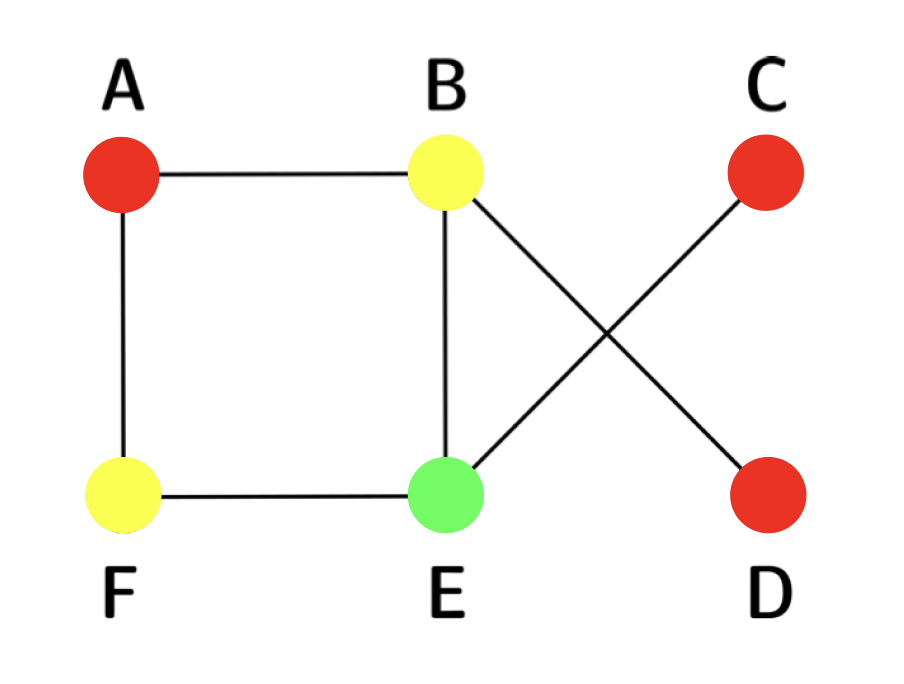
\includegraphics[scale=0.5]{coloring.png}
%      \caption{Coloring of the graph.}
% \end{figure}

% \begin{figure}[htb]
%     \qquad
%     \begin{minipage}{.4\textwidth}
%         \centering
%         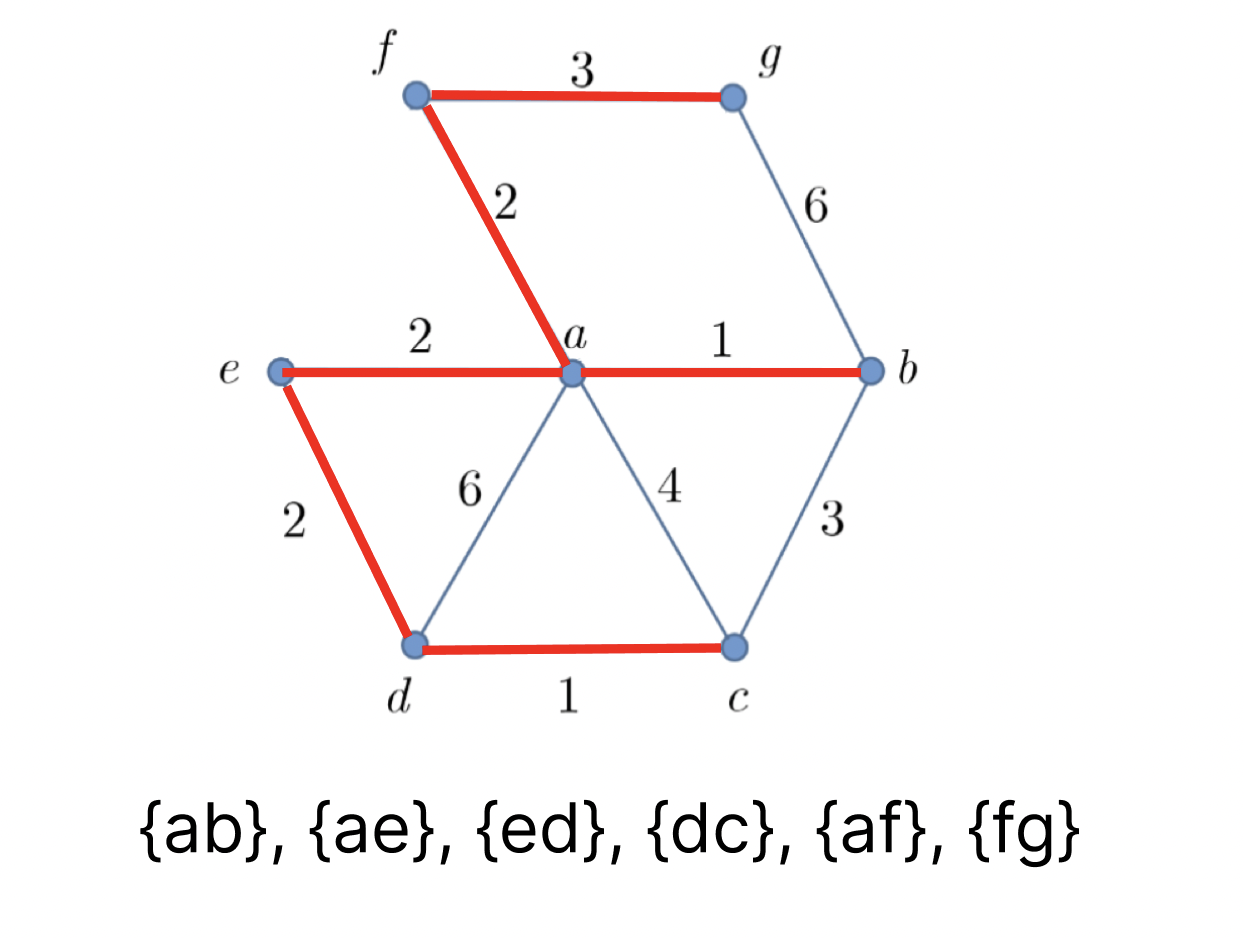
\includegraphics[scale=0.35]{prims.png}
%         \caption{}
%     \end{minipage}    
%     \qquad
%     \begin{minipage}{.4\textwidth}
%         \centering
%         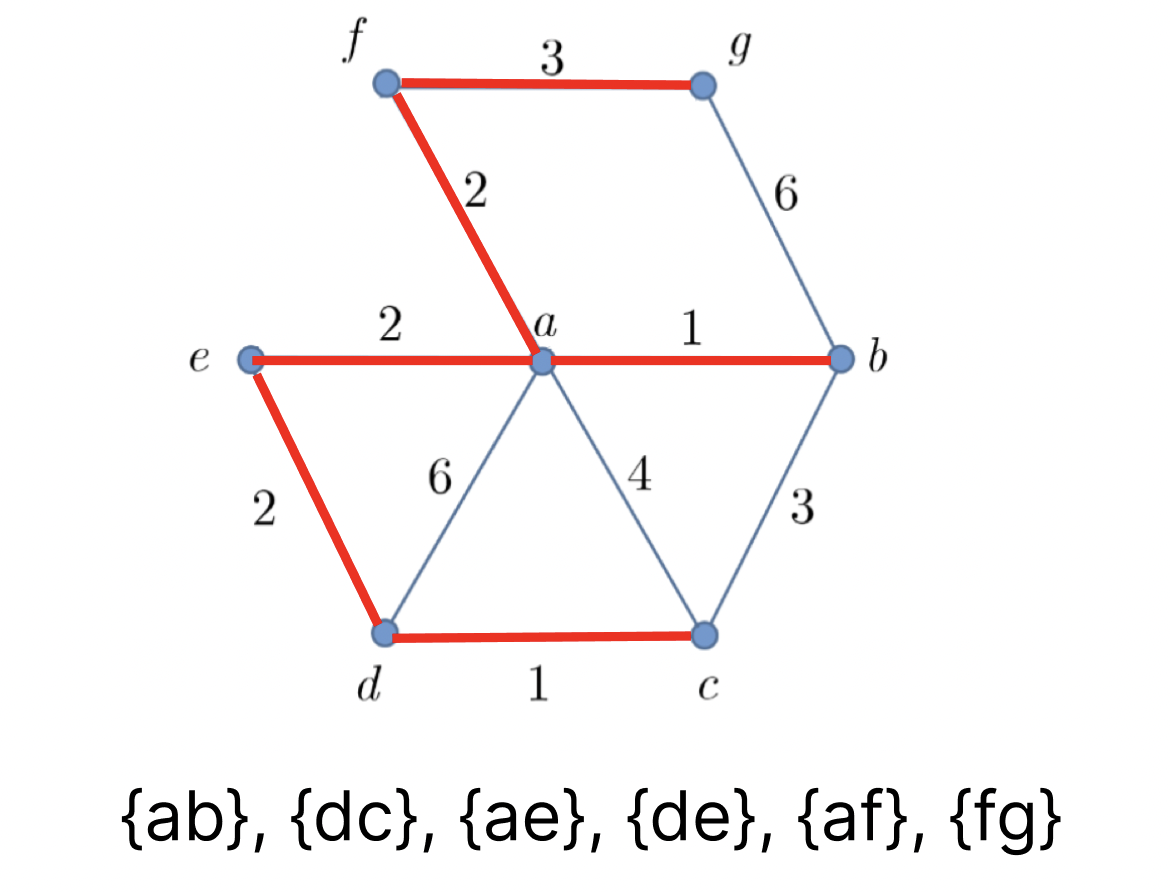
\includegraphics[scale=0.35]{kruskal.png}
%         \caption{}
%     \end{minipage}        
% \end{figure} 

\newtheorem{thm}{Theorem}
\newtheorem{proposition}[thm]{Proposition}
\newtheorem{corollary}[thm]{Corollary}
\newtheorem{lemma}[thm]{Lemma}

\newcommand*{\Var}{\ensuremath{\mathrm{Var}}}
\newcommand*{\Cov}{\ensuremath{\mathrm{Cov}}}
\newcommand*{\Corr}{\ensuremath{\mathrm{Corr}}}
\newcommand*{\Bias}{\ensuremath{\mathrm{Bias}}}
\newcommand*{\MSE}{\ensuremath{\mathrm{MSE}}}
\newcommand*{\range}{\ensuremath{\mathrm{range}}\,}
\newcommand*{\spann}{\ensuremath{\mathrm{span}}\,}
\newcommand*{\nul}{\ensuremath{\mathrm{null}}\,}
\newcommand*{\dom}{\ensuremath{\mathrm{dom}}\,}
\renewcommand*{\implies}{\ensuremath{\Longrightarrow}}
\renewcommand*{\impliedby}{\ensuremath{\Longleftarrow}}
\newcommand*{\Z}{\ensuremath{\mathbb{Z}}}
\newcommand*{\Q}{\ensuremath{\mathbb{Q}}}
\newcommand*{\R}{\ensuremath{\mathbb{R}}}
\newcommand*{\F}{\ensuremath{\mathbb{F}}}
\newcommand*{\C}{\ensuremath{\mathbb{C}}}
\newcommand*{\N}{\ensuremath{\mathbb{N}}}
\newcommand*{\E}{\ensuremath{\mathds{E}}}
\renewcommand*{\P}{\ensuremath{\mathds{P}}}
\newcommand*{\p}{\ensuremath{\mathcal{P}}}

% title information
\title{Math 104 HW10}
\author{Neo Lee}
\date{11/17/2023}

\setstretch{1.15}
% main content
\begin{document} 

% placing title information; comment out if using fancyhdr
\maketitle 

\subsection*{Exercise 25.7}
\begin{proposition}
    $\sum_{n=1}^{\infty}\frac{1}{n^2}\cos nx$ converges uniformly on $\R$ to a continuous 
    function.
\end{proposition}
\begin{proof}
    Let $(M_n)=\frac{1}{n^2}$ and $g_n=\frac{1}{n^2}\cos nx$, then $|g_n|\le \frac{1}{n^2}=M_m$ 
    because $|\cos nx|\le 1$. Since $\sum_{n=1}^{\infty}\frac{1}{n^2}$ converges by 
    \emph{Theorem 15.1}, by \emph{Weierstrass M-test}, $\sum_{n=1}^{\infty}\frac{1}{n^2}\cos nx$
    converges uniformly on $\R$. Since $\cos$ is continuous, a constant times a continuous function 
    $g_n=\frac{1}{n^2}\cos nx$ for $n\in\N$ is continuous. By \emph{Theorem 25.5}, 
    $\sum_{n=1}^{\infty}\frac{1}{n^2}\cos nx$ is continuous.
\end{proof}

\newpage
\subsection*{Exercise 25.10}
\begin{proposition}\indent
    \begin{enumerate}[label=\textbf{(\alph*)}]
        \item $\sum\frac{x^n}{1+x^n}$ converges for $x\in[0,1)$.
        \item The series converges uniformly on $[0,a]$ for each $a\in(0,1)$.
        \item Does the series converge uniformly on $[0,1)$? Explain.
    \end{enumerate}
\end{proposition}
\begin{proof}\indent
    \begin{enumerate}[label=\textbf{(\alph*)}]
        \item For $x\in(0,1)$, 
        \begin{align*}
            & \left|\frac{a_{n+1}}{a_n}\right|=\left|\frac{x^{n+1}}{1+x^{n+1}}\cdot \frac{1+x^n}{x^n}\right| = 
            \left|\frac{1+x^n}{1+x^{n+1}}\cdot x\right| \\
            & \lim x^{n+1} = \lim x^n = 0 \implies \lim \left|\frac{1+x^n}{1+x^{n+1}}\cdot x\right| 
            = \frac{1}{1}\cdot x = x < 1 \\
            & \implies \lim\sup|a_{n+1}/a_n|=\lim|a_{n+1}/a_n|<1.
        \end{align*}
        By \emph{Ratio Test}, $\sum\frac{x^n}{1+x^n}$ converges for $x\in(0,1)$. 
        For $x=0$, the series obviously converges to 0. Hence, 
        $\sum\frac{x^n}{1+x^n}$ converges for $x\in[0,1)$.

        \textbf{Alternatively,} notice $\frac{x^n}{1+x^n}\le x^n$ for $x\in[0,1)$. By 
        \emph{Comparison Test} with $\sum x^n$, which converges because $|x|<1$, the series 
        converges.

        \item We show that the series satisfies Cauchy Criterion uniformly on $[0,a]$. Notice for 
        all $n\ge m$, $$\left|\sum_{k=m}^{n}\frac{x^k}{1+x^k}\right|\le 
        \left|\sum_{k=m}^{n}x^k\right|\le \left|\sum_{k=m}^{n}a^k\right|,$$
        which means we only need to find $N$ such that for all $n\ge m> N$,
        $$\left|\sum_{k=m}^{n}a^k\right|<\epsilon.$$ We already know such $N$ exists 
        because $\sum a^k$ converges as $|a|<1\implies\sum a^k$ satisfies Cauchy Criterion
        $\implies$ such $N$ exists. Hence, $\sum\frac{x^n}{1+x^n}$ converges uniformly on $[0,a]$.

        \item No, the series does not converge uniformly on $[0,1)$. 
        Denote $f_n(x) = \sum_{k=0}^{n}\frac{x^k}{1+x^k}$. Assume for the sake of contradiction that 
        the series converges uniformly on $[0,1)$, then there exists $N$ such that for all $n> N$,
        $$|f_n(x)-f(x)|<\epsilon \qquad \text{for all $x\in[0,1)$},$$ where 
        $$f(x)= \sum_{k=0}^{\infty}\frac{x^k}{1+x^k}.$$
        Specifically for $n=N+1$
        $$\left|\sum_{k=0}^{n}\frac{x^k}{1+x^k}-\sum_{k=0}^{\infty}\frac{x^k}{1+x^k}\right|
        = \left|\sum_{k=N+2}^{\infty}\frac{x^k}{1+x^k}\right|<\epsilon \qquad \text{for all $x\in[0,1)$}.$$
        Now denote $g(x)=\left|\sum_{k=N+2}^{\infty}\frac{x^k}{1+x^k}\right|$. However, notice 
        as $x\to1$, $g(x)\to \infty$. Therefore, there always exists $x\in[0,1)$ such that
        $g(x)>\epsilon$, which is a contradiction. Hence, the series does not converge uniformly
        on $[0,1)$.
        
        
    \end{enumerate}
\end{proof}

\newpage
\subsection*{Exercise 28.4}
\begin{proposition}
    Let $f(x)=x^2\sin \frac{1}{x}$ for $x\neq 0$ and $f(0)=0$.
    \begin{enumerate}[label=\textbf{(\alph*)}]
        \item $f$ is differentiable at each $a\neq 0$ and calculate $f'(a)$. Prove using 
        \emph{Theorem 28.3, 28.4}.
        \item $f$ is differentiable at $x=0$ and $f'(0)=0$. Prove using the definition.
        \item $f'$ is not continuous at $0$.
    \end{enumerate}
\end{proposition}
\begin{proof}
    \begin{enumerate}[label=\textbf{(\alph*)}]
        \item 
        We have $\frac{1}{x}$ is differentiable for $x\neq 0$ due to \emph{Example 4}, and $\sin$ is differentiable, 
        then by \emph{Theorem 28.4}, $\sin\frac{1}{x}$ is differentiable at $a\neq 0$ and the derivative 
        is $-\cos \frac{1}{x}\cdot \frac{1}{x^2}$. We also know $x^2$ is differentiable due to 
        \emph{Example 3}. By \emph{Theorem 28.3 (iii)}, $f$ is differentiable at $a\neq 0$ and
        $$f'(a)=2a\sin \frac{1}{a}-\cos \frac{1}{a}.$$

        \item \begin{align*}
            f'(0) & = \lim_{x\to0} \frac{f(x)-f(0)}{x-0} = 
            \lim_{x\to0} \frac{x^2\sin \frac{1}{x}}{x} = 
            \lim_{x\to0} x\sin \frac{1}{x},
        \end{align*}
        which we have shown in previous homework that the limit is 0 because 
        we can take $\delta = \epsilon$, then since $|\sin\frac{1}{x}|\le 1$ for $x\neq 0$,
        $$|x|<\delta\implies \left|x\sin\frac{1}{x}\right|<\delta=\epsilon.$$

        \item Consider the sequence $(x_n)=\frac{1}{n}$, which has limit equal to 0. Then, 
        $$f'(x_n) = \frac{2}{n}\sin n - \cos n.$$ Assume for the sake of contradiction that
        $\lim f'(x_n)=0$, which means there exists $N$ such that for all $n> N$,
        $$\left|\frac{2}{n}\sin n - \cos n\right|<\epsilon.$$ More concretely, take $\epsilon = 0.1$.
        Now, notice $\lim \frac{2}{n}\sin n=0$
        because $\left|\frac{2}{n}\sin n\right|\le \left|\frac{2}{n}\right|$, which has a limit of 0. 
        This means there exists $M$ such that for all $n> M$, $\left|\frac{2}{n}\sin n\right|<\epsilon$.
        However, notice there exists $n> \max\{N,M\}$ such that $\cos n > 2\epsilon$, which means 
        $$\left|\frac{2}{n}\sin n - \cos n\right|>\epsilon,$$
        which is a contradiction. Hence, $\lim f'(x_n)\neq 0$, which means $f'$ is not continuous 
        at 0.

    \end{enumerate}
\end{proof}

\newpage
\subsection*{Exercise 28.8}
\begin{proposition}
    Let $f(x)=x^2$ for $x$ rational and $f(x)=0$ for $x$ irrational.
    \begin{enumerate}[label=\textbf{(\alph*)}]
        \item $f$ is continuous at $x=0$.
        \item $f$ is discontinuous at each $x\neq 0$.
        \item $f$ is differentaible at $x=0$.
    \end{enumerate}
    \begin{proof}\indent
        \begin{enumerate}[label=\textbf{(\alph*)}]
            \item Take $\delta = \min\{1, \epsilon\}$, then for all $x$ irrational such that
            $|x-0|<\delta \implies |f(x)-f(0)|=|0-0|<\epsilon$. Now, for all $x$ rational such that 
            $|x-0|<\delta, \implies |f(x)-f(0)|=|x^2| < \epsilon^2<\epsilon$ when $\epsilon <1$, and 
            $|f(x)-f(0)|=|x^2|<1\le \epsilon$ when $\epsilon \ge 1$.

            \item For $x_0\neq 0$, we can take $\epsilon = \frac{x_0^2}{2}$, then for all $\delta>0$,
            there exists $x\in (x_0-\delta, x_0+\delta)$ and $|x_0|<|x|$ that is rational and $y\in (x_0-\delta, x_0+\delta)$ that is
            irrational. If $x_0$ is irrational, then $|x-x_0|<\delta$ but $|f(x)-f(x_0)|=|x^2|>|x_0^2|>\epsilon$.
            If $x_0$ is rational, then $|y-x_0|<\delta$ but $|f(y)-f(x_0)|=|x_0^2|>|x_0^2/2|=\epsilon$.

            \item 
            \begin{align*}
                \frac{f(x)-f(0)}{x-0} & = \frac{x^2}{x} =x \qquad \text{if $x$ is rational} \\
                \frac{f(x)-f(0)}{x-0} & = \frac{0}{x} = 0 \qquad \text{if $x$ is irrational}.
            \end{align*}
            Then $$\lim f'(x) =\lim \frac{f(x)-f(0)}{x-0} = 0,$$
            because we can take $\delta = \epsilon$ and $|x|<\delta\implies |x|<\epsilon$.
        \end{enumerate}
    \end{proof}
\end{proposition}

\newpage
\subsection*{Exercise 28.14}
\begin{proposition}
    Suppose $f$ is differentiable at $a$,
    \begin{enumerate}[label=\textbf{(\alph*)}]
        \item $\lim_{h\to0}\frac{f(a+h)-f(a)}{h}=f'(a)$,
        \item $\lim_{h\to0}\frac{f(a+h)-f(a-h)}{2h}=f'(a).$
    \end{enumerate}
\end{proposition}
\begin{proof}\indent
    \begin{enumerate}[label=\textbf{(\alph*)}]
        \item Notice we can write $x=a+h$, then $x-a=h$ and $x\to a\equiv h\to 0$. Then,
        \begin{align*}
            \lim_{h\to0}\frac{f(a+h)-f(a)}{h} & = \lim_{x\to a}\frac{f(x)-f(a)}{x-a} = f'(a).
        \end{align*}

        \item
        \begin{align*}
            \lim_{h\to0}\frac{f(a+h)-f(a-h)}{2h} & = 
            \lim_{h\to0}\frac{f(a+h)-f(a)+f(a)-f(a-h)}{2h} \\
            & = \lim_{h\to0}\frac{f(a+h)-f(a)}{2h} + \frac{f(a)-f(a-h)}{2h} \\
            & = \lim_{h\to0}\frac{1}{2}\left(\frac{f(a+h)-f(a)}{h} + \frac{f(a)-f(a-h)}{h}\right) \\
            & = \lim_{h\to0}\frac{1}{2}\left(\frac{f(a+h)-f(a)}{h} + \frac{f(a-h)-f(a)}{-h}\right).
        \end{align*}
        Now notice we can write $x=a-h$, then $x-a=-h$ and $x\to a\equiv h\to 0$. Then,
        $$\lim_{h\to0}\frac{f(a-h)-f(a)}{-h} = \lim_{x\to a}\frac{f(x)-f(a)}{x-a} = f'(a).$$
        We know $f$ is differentiable at $a$, which means $f'(a)=L$ for finite $L$, then 
        $$\lim_{h\to0}\frac{f(a+h)-f(a)}{h} = \lim_{h\to0}\frac{f(a-h)-f(a)}{-h} = L,$$
        and \begin{align*}
            \lim_{h\to0}\frac{1}{2}\left(\frac{f(a+h)-f(a)}{h} + \frac{f(a-h)-f(a)}{-h}\right) & =
            \frac{1}{2}\left(\lim_{h\to0}\frac{f(a+h)-f(a)}{h} + \lim_{h\to0}\frac{f(a-h)-f(a)}{-h}\right) \\
            & = \frac{1}{2}\left(L+L\right) = L = f'(a).
        \end{align*}
    \end{enumerate}
\end{proof}


\end{document}
